\documentclass[../main]{subfiles}

\input{chapter_header.tex}

\begin{document}

\chapter{TinyML Modeling Structure} \label{chp:}

TinyML enables the deployment of machine learning models directly on microcontrollers like the ESP32. In the GMU, TinyML is used to identify plant growth stages from captured images without requiring cloud computation.

\subsection{Workflow}
\begin{enumerate}
    \item \textbf{Data Collection:} Images of plant seedlings are collected using the ESP32-CAM or public datasets (e.g., Plant Seedlings Dataset from Kaggle). Each image is labeled according to stages: Germination, Sprouting, Early Growth, Mature.
    \item \textbf{Data Preprocessing:} Images are resized (e.g., 96×96 pixels), normalized, and augmented (rotation, brightness change, cropping) to improve generalization.
    \item \textbf{Model Training:} The CNN model is trained using TensorFlow/Keras with layers such as Convolution, Pooling, and Dense layers, ending with a Softmax classifier.
    \item \textbf{Model Optimization:} The trained model is quantized (8-bit integer) using TensorFlow Lite for Microcontrollers to reduce memory footprint and improve inference speed.
    \item \textbf{Deployment:} The optimized \texttt{.tflite} model is flashed onto the ESP32 for on-device inference.
    \item \textbf{Output:} The model classifies the captured image into a growth stage category and sends results to the monitoring interface.
\end{enumerate}

\begin{figure}
    \centering
    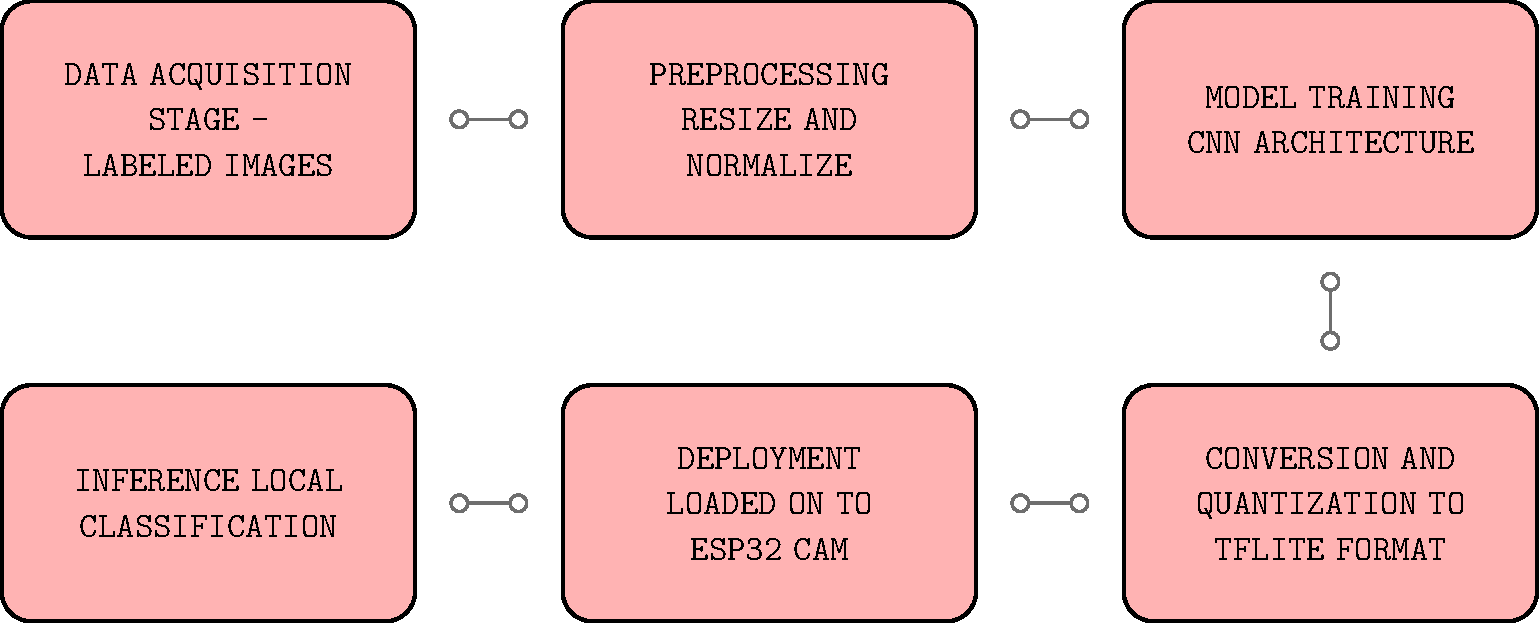
\includegraphics [
        width = 0.7\textwidth,
        max width = \IGXMaxWidth,
        max height = \IGXMaxHeight,
        \IGXDefaultOptionalArgs,
    ] {tikzpics/endAbsTinyMLWorkflow.pdf}
    \captionof{figure} {TinyML Workflow for GMU: Data Collection to Deployment}
    \label{fig:}
\end{figure}

% \begin{figure}[H]
%     \centering
%
%     \begin{tikzpicture}
%
%         \draw [
%             thick,
%             rounded corners = 0.3cm,
%         ]
%         (0, 0) coordinate (origin)
%
%         (2, 2) coordinate (origin)
%
%         (origin) rectangle ++(1, 1)
%
%         (0, 0) -- (2, 0)
%         ;
%
%     \end{tikzpicture}
%
%     %
%     % \includegraphics[width=0.85\textwidth]{example-image}
%     % % \includegraphics[width=0.85\textwidth]{tinyml_workflow.png}
%     \caption{TinyML Workflow for GMU: Data Collection to Deployment}
% \end{figure}

\subsection{Model Architecture Example}

\begin{table}[H]
    \centering
    \begin{tabularx} {\textwidth} {
            >{\raggedright}m{5cm}
            >{\centering}X
            >{\centering \arraybackslash}X
        }

        \toprule
        \textbf{Layer Type} & \textbf{Output Shape} & \textbf{Parameters} \\
        \midrule

        Input Image (96×96×3) & - & - \\
        Conv2D (16 filters, 3×3) & 94×94×16 & 448 \\
        MaxPooling2D (2×2) & 47×47×16 & 0 \\
        Conv2D (32 filters, 3×3) & 45×45×32 & 4,640 \\
        Flatten & - & 0 \\
        Dense (64 units, ReLU) & 64 & 4,147,264 \\
        Output (Softmax, 4 units) & Growth Stage & 260 \\
        \bottomrule
    \end{tabularx}
    \caption{Example CNN Architecture for TinyML Model.}
\end{table}

\subsection{Expected Model Performance}

\begin{table}[H]
    \centering
    \begin{tabularx} {\textwidth} {
            >{\raggedright \arraybackslash}X
            >{\raggedright \arraybackslash}X
        }
        \toprule
        \textbf{Metric} & \textbf{Value} \\ \midrule
        Accuracy & 92–95\% \\
        Model Size & $<$ 1 MB \\
        Inference Time & $\sim$150 ms \\
        Power Consumption & $<$ 1 W \\
        Deployment Target & ESP32-CAM (TFLite Micro) \\
        \bottomrule
    \end{tabularx}
    \caption{Expected TinyML Model Performance.}
\end{table}

\section{Integration with GMU}
The TinyML model runs in synchronization with the mechanical movement of the GMU. For every scan position, the camera captures and classifies an image. The classified growth stage is stored and transmitted along with environmental data such as temperature and humidity, ensuring seamless integration of mechanical and AI-based monitoring.

\section{Expected Outputs}
\begin{itemize}
    \item Smooth camera movement across the tray.
    \item Clear captured images of seedlings.
    \item Real-time classification of plant growth stages.
    \item Visualization of stage-wise growth progress on the monitoring dashboard.
\end{itemize}

\section{Applications}
\begin{itemize}
    \item Automated agricultural monitoring.
    \item Seed germination and plant growth research.
    \item Smart greenhouse systems.
    \item Embedded TinyML educational demonstrations.
\end{itemize}

\section{Future Enhancements}
\begin{itemize}
    \item Integration of multi-axis scanning for 3D growth mapping.
    \item Use of advanced CNN architectures such as MobileNet or EfficientNet for higher accuracy.
    \item Implementation of adaptive lighting control for uniform image capture.
    \item Integration with cloud dashboards for long-term data analytics.
\end{itemize}

\section{Conclusion}
The GMU demonstrates the successful integration of mechatronics, embedded systems, and TinyML for plant growth monitoring. It showcases how low-cost microcontrollers can perform on-device intelligence, enabling efficient, real-time agricultural automation.



\end{document}
